\chapter{Introduction}
\section{C$_4$ Photosynthesis \& C$_4$ rice}

\begin{wrapfigure}{r}{0.5\textwidth}%
	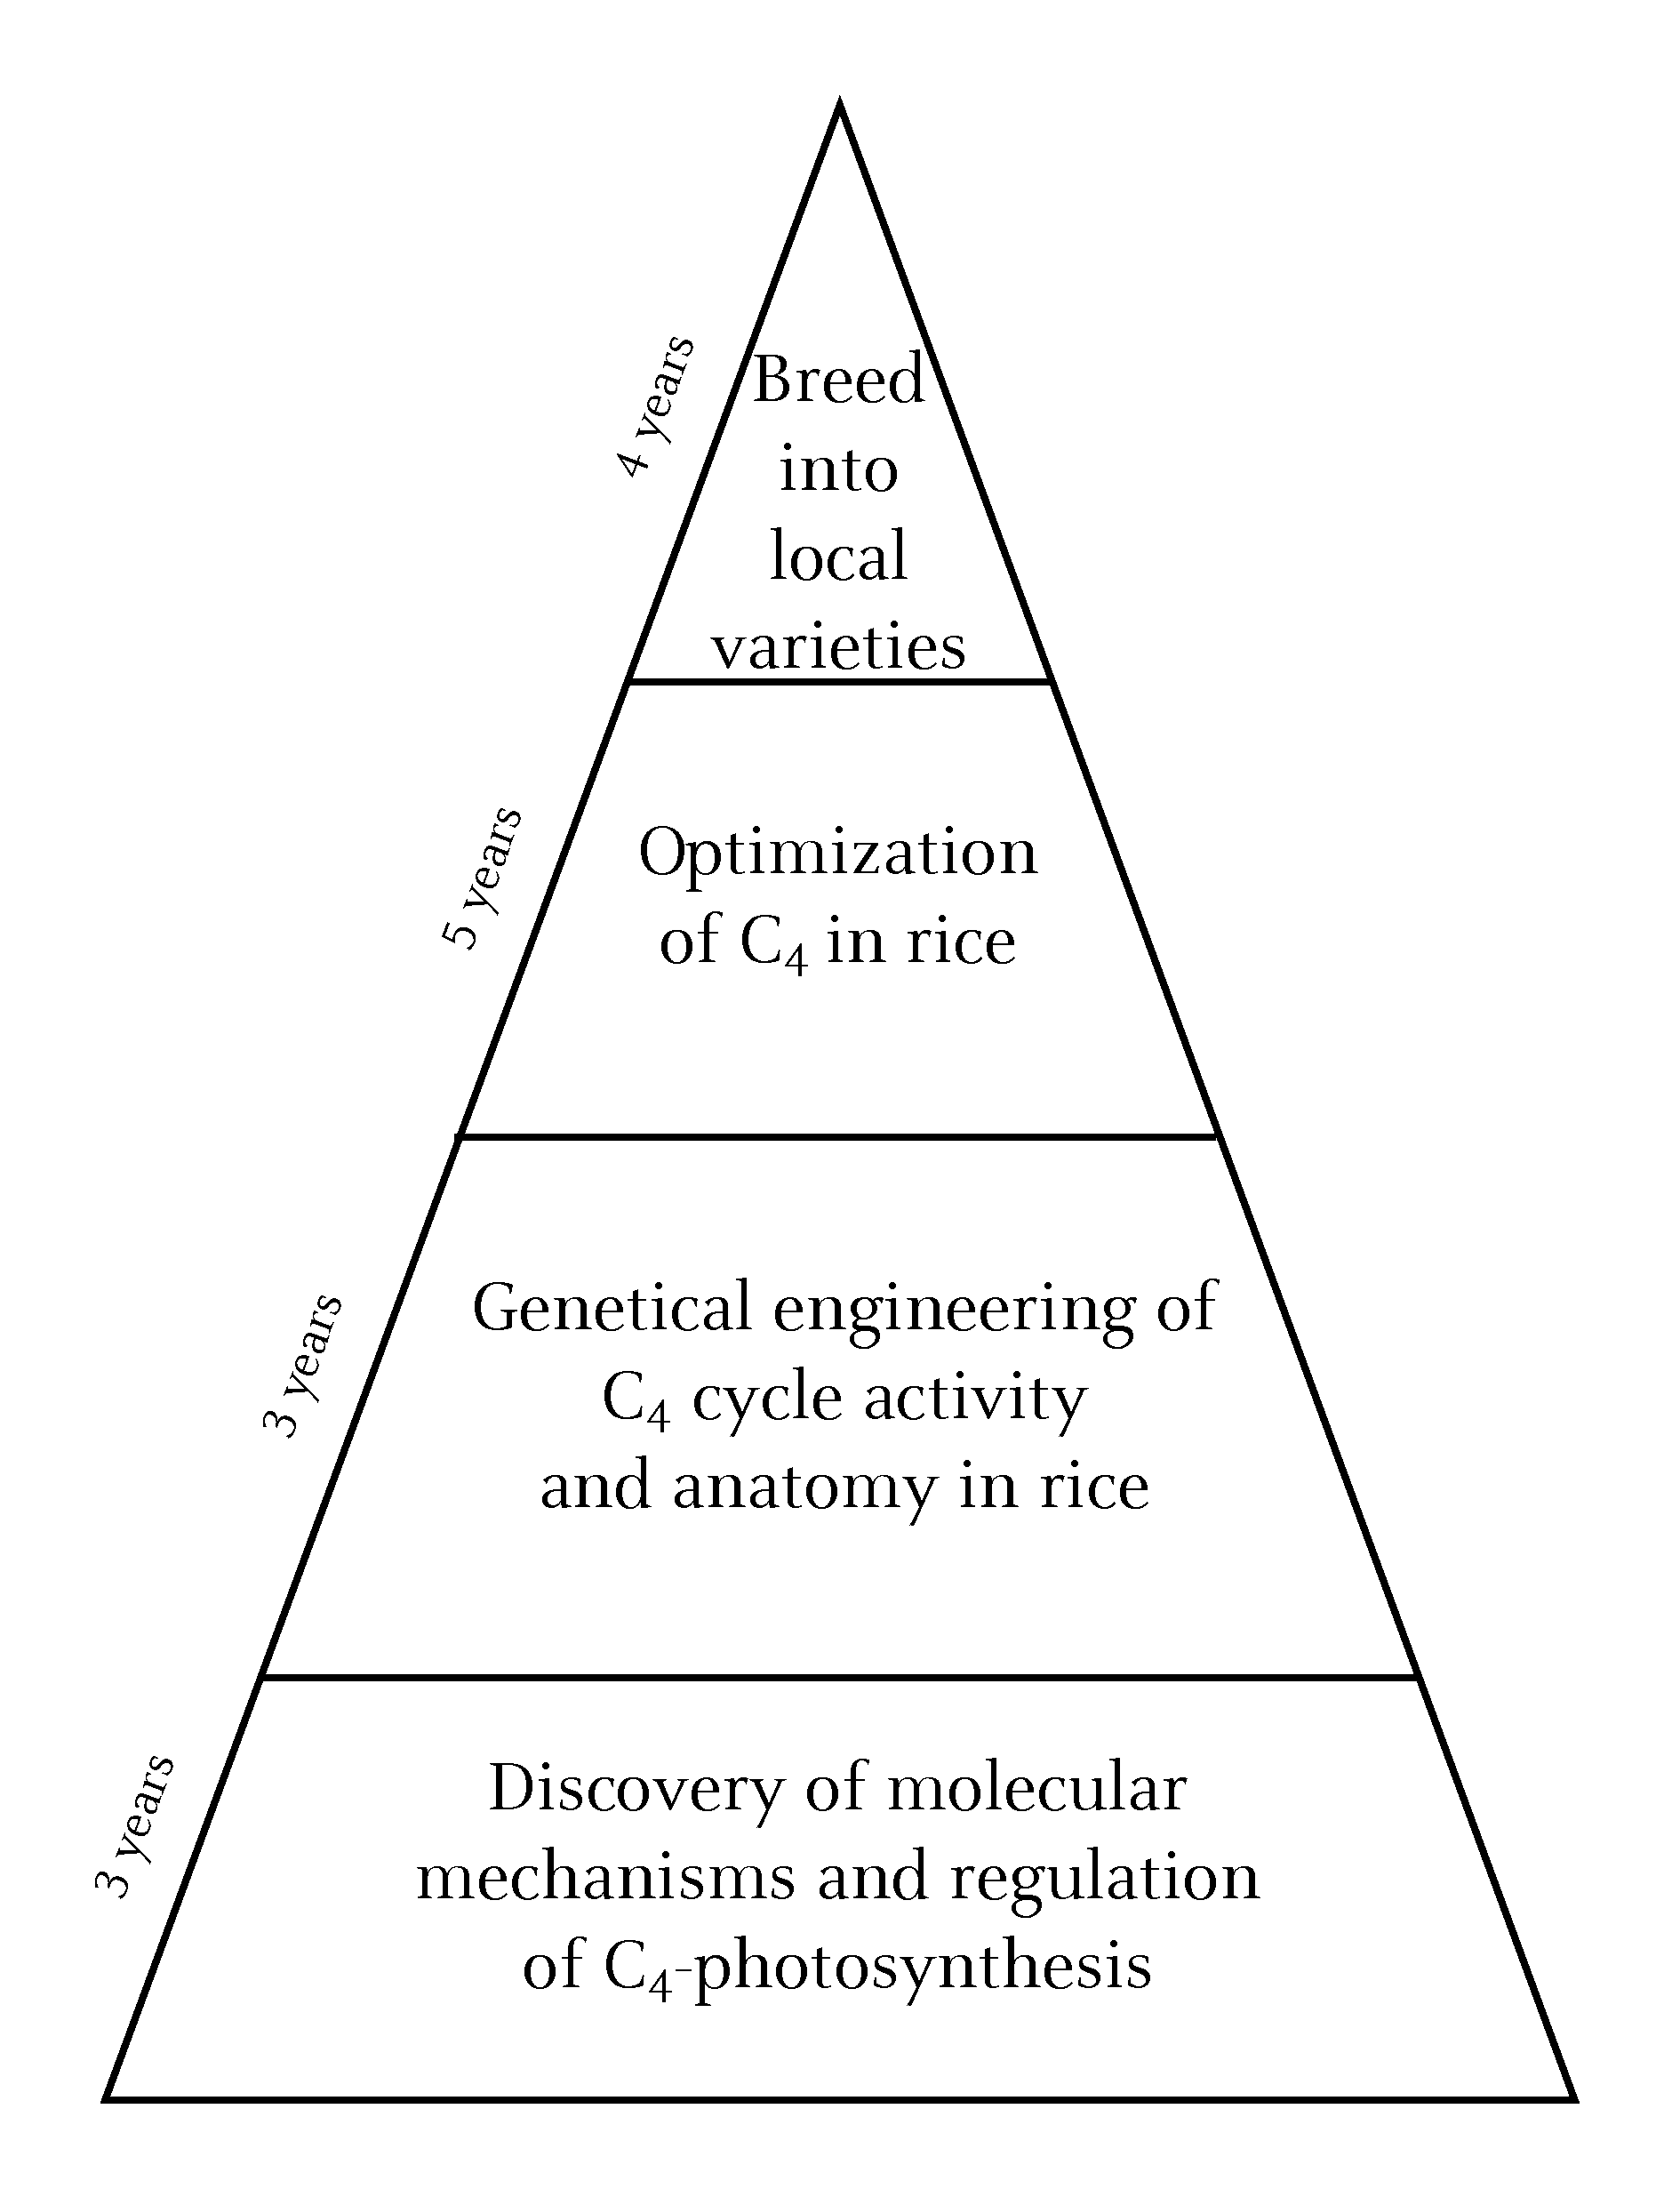
\includegraphics[width=0.48\textwidth]{images/C4_roadmap}%
	\caption{Roadmap for the C$_4$-Rice Project \href{http://c4rice.irri.org}{(c4rice.irri.org)}}%
	\label{fig:c4rice_roadmap}%
\end{wrapfigure}

Around one billion people in the world feed on rice.
Rice is a cheap, non-perishable crop.
However, with growing population sizes the demand for rice increases, as well.
Now, C$_4$ photosynthesis is considered a very promising trait to cope with this demand by increasing yield.
\subsection{C$_3$ Photosynthesis}
Photosynthesis describes the conversion of CO$_2$ and light energy to sugars.
The primary fixation of CO2 is catalysed by \ac{RuBisCO}.
CO$_2$ is attached to ribulose-1,5-bisphosphate (5C) yielding two molecules of phosphoglycerate (3C), hence the name C$_3$ photosynthesis.
However, a side reaction to \ac{RuBisCO} fixing CO$_2$ is the fixation of oxygen.
The resulting molecule phosphoglycolate needs to be recycled at the loss of CO$_2$ and energy.
This process, called photorespiration reduces the overall efficiency.
Carbon fixation in plants performing only C$_3$ photosynthesis is, therefore, dependent on the CO$_2$ availability.
\subsection{C$_4$ photosynthesis}
C$_4$ photosynthesis is a trait that has evolved independently over 60 times throughout the plant kingdom.
Within the \species{Poaceae} (grasses) the evolutionary origins of C$_4$ photosynthesis are confined within the PACMAD clade.
Plants performing C$_4$ photosynthesis have evolved to avoid photorespiration and thus reduce energy loss.
The mechanism to avoid photorespiration consists of changes in metabolism as well as cell architecture.
A spatial separation of primary carbon fixation and fixation by \ac{RuBisCO} has evolved by confining the expression of \ac{RuBisCO} to the bundle sheath cells.
In parallel primary CO$_2$ fixation is catalysed by PEP carboxylase in the mesophyll cells.
The transfer of fixed CO$_2$ from mesophyll to bundle sheath is carried out by transfer acids, such as malate or aspartate.
After transfer to the bundle sheath, the fixed CO$_2$ is released again.
Thus the two step fixation of C$_4$ photosynthesis increases the CO$_2$ concentration in the vicinity of \ac{RuBisCO} and suppresses the need for photorespiration.
As a consequence, less \ac{RuBisCO} enzyme is needed.
Therefore, C$_4$ plants present a higher efficiency.
%More details wouldn't hurt
\subsection{C$_4$ rice}
While the demand for food is growing the area accessible to agriculture is shrinking.
One approach to induce a second green revolution is genetically engineering rice into a C$_4$ plant.
Expectations are not only that the yield will increase in current environments, but also rice will become accessible to more climate regions.
The International Rice Research Institute has laid out a roadmap to reach this goal.
In general, the project can be summarised as: Understand, Imitate, Optimise, and Breed.
That means, as depicted in figure \ref{fig:c4rice_roadmap}, they suggest a coordinated research effort over the next 15 years.
Starting with a detailed analysis of all molecular components involved in C$_4$.
Followed by engineering efforts to establish a C$_4$ like metabolism in rice.
Subsequently improving the cycle yield within rice transgenics.
Finally crossing rice transgenics with existing rice cultivars to generate location-adapted C$_4$ rice plants.
In terms of this roadmap, my work focuses on the analysis of the C$_4$-cycle within grasses.
It aims at describing a set of parts and interconnections in order to build a blueprint for re-engineering C$_4$ photosynthesis.
Thus the main driving force of my work was the question: 
\formatquote{Which transcripts are involved in creating the difference between C$_3$ and C$_4$ photosynthesis in two closely related grass species?}

\section{Next-Generation Sequencing}
Sequencing DNA fragments has already been described in the late 70s.
One chemical approach, as well as an approach based on PCR was presented.
Despite optimisations, like fluorescent dyes and capillary electrophoresis, the throughput of these traditional approaches was rather low.
The second generation of sequencing approaches includes the ones used in this work.
Characteristic for these sequencing approaches is that they provide a high sequence throughput and in contrast to the first generation allow for a reliable estimation of sequence abundance in the sample.
A new third generation of sequencing platforms has been introduced in recent years.
As a major difference, third generation sequencing allows for sequencing of actual DNA molecules and therefore shows no bias of the amplification steps, some second generation sequencing methods suffered.
The reliability of these platforms is still controversially discussed.

\subsection{Sequencing platforms used during PhD project}
\subsubsection{Pyrosequencing (454)}
Massively parallel pyrosequencing is an approach that has been commercially launched by 454 Life Sciences and was later acquired by Roche.
DNA fragments are randomly distributed over a picotiter plate and subsequently amplified in the picoliter wells.
This renders the DNA immobile and keeps the position of each fragment consistent during sequencing.
Chemically the sequencing approach detects the pyrophosphate, which is released upon insertion of a nucleotide during DNA synthesis inside of each well.
A combined sulfurylase:luciferase enzyme creates light emission for each pyrophosphate molecule released.
Therefore, a CCD camera module can capture the amount of light generated per well.
To sequence, the machine repeatedly adds dNTPs separately, so the light information collected is assigned to a certain nucleotide for each fragment.
This sequencing approach suffers from long homopolymer stretches, because the light intensity detection becomes ambiguous.
Read lengths of up to 800 bp are possible on GS FLX with Titanium chemicals.
The number of reads is about a million per picotiter plate.

\subsubsection{SOLiD}
Sequencing by ligation has been introduced by Applied Biosystems (now Life Technologies) with the SOLiD platform.
In this approach a fluorescent dye labeled oligonucleotide is binding two nucleotides of the template strand.
The readout is a color value.
One of the two bases is ligated and the process repeats with the position shifted by one.
This way, each base is read twice, which increases the accuracy to 99.8\%.
Colorspace sequences can be converted to basespace by interpreting the sequence of colors as base-pairings.
Even though this increases accuracy, one skipped readout is sufficient to invalidate the rest of the read.
In other words, the information of each base is dependent on the information of the previous base.
SOLiD sequencing can generate up to 30G bases with a maximum length of 85 bp.

\subsubsection{Illumina}
The use of modified ddNTPs to identify inserted bases during strand synthesis categorises Illumina sequencing as sequencing by synthesis technology.
The provided nucleotides are enhanced with a cleavable fluorescent dye and a removable blocking group.
The blocking group prevents multiple base insertions and leads to a one base at a time readout.
A CCD camera captures the light emission of the fluorescent labels during laser excitation.
Because of the blocking groups, Illumina sequencing has a fixed read length.
Currently, the output of Illumina can reach up to 600G bases with a read length of up to 2x150 bp.
Comparing the three sequencing technologies, Illumina has the highest rate of error with up to 2\%.
Working towards quantitative as well as qualitative sequence data:
\formatquote{What is the best sequencing approach to answer my experimental question?}

%Following paragraph might fit better into conclusions
\subsubsection{What is the best platform?}
Choosing a sequencing platform is highly dependent on the experimental design.
Sequencing \foreignword{de novo}, i.e. without a reference genome, is considered easier if the read length is higher.
Whereas, analysing statistical differences in gene regulation benefits from a high number of reads.
Finally, the costs, accuracy, and availability of analysis software need to be considered.
Therefore, there are different best platforms for a single use-case, but not a single best platform for all use-cases.

\subsection{Assembly \& mapping}
%I will first go to lunch
%I'm back from lunch, let's rock
High throughput sequencing technologies have arisen only recently.
The rapid changes and improvements in sequencing technologies are accompanied by changes in big data analytics, as well.
Therefore, the computational methods available for traditional sequencing need to be re-validated.
Part of the work presented here focused on this validation especially towards \foreignword{de novo} transcriptome sequencing, where the outcome is unpredictable.
\subsubsection{\foreignword{De novo} assembly}
In contrast to reference-based sequence assembly, where the read sequences are matched to a known genome, in \foreignword{de novo} assembly, the full-length information for a gene must be extracted from the read information alone.
Two conceptually different solutions are currently known: \ac{OLC} and \ac{DBG} assembly.

In \ac{OLC} assemblers all reads are compared to each other (pairwise or grouped) and assembled into contigs, where overlaps exist.
This method is optimised for few and long sequences.
The number of comparisons, hence the runtime, as well as the memory consumption increase more than linear with read numbers.
Algorithms based on the \ac{OLC} principle differ in the pre-selection of reads to compare or in the error tolerance.

\ac{DBG} assemblers employ graph theory to solve the overlap problem.
That means, a read is represented by a sequence of k-mer nodes, for which every node overlaps in k-1 positions with the neighboring nodes.
This approach transfers the problem of finding overlaps in all against all reads to finding supported paths through the graph.
\ac{DBG} assemblers can handle much higher read numbers because memory consumption and computational power required are dependent on the number of unique k-mers used and not necessarily the number of reads.
With many algorithms at hand:
\formatquote{What is the best way to assemble the generated 454 \& Illumina reads to get reliable transcript sequences?}

\subsubsection{Read mapping}
%cross-species problem, error tolerance, contig mapping bias.
In order to get quantitative information about gene expression, the sequenced reads need to be assigned to genes.
Multiple approaches have been developed for read mapping to a reference genome.
One of the most commonly used mapping algorithms to achieve this is bowtie.
Bowtie is optimised for mapping speed of nearly perfect sequences.
However, this algorithm does not work on \foreignword{de novo} sequencing data.
In \foreignword{de novo} approaches a reference genome is not available or not used on purpose.
Thus, the read mapping is transferred to a reference sequence of a species that is closely related to the sequenced species.
Even short evolutionary distances between species can account for many exchanges in the nucleotide sequence.
Thus, mapping software like bowtie is unable to match many reads.
Traditional programs, such as BLAST or BLAT, which are not optimised for speed, allow for mapping in proteinspace, i.e. translated nucleotide sequence mapped in all possible frames.
Since there is redundancy in codon to amino acid translation, proteinspace mapping is not affected by synonymous base changes, and thus lenient about the actual nucleotide sequence.
% more error tolerance, contig mapping bias
Hence, the question:
\formatquote{What is the best mapping approach for this study?}

\subsection{Statistics}
%t-Test, Fisher's Exact Test, DEGSeq, DESeq
One of the main challenges in statistics on transcriptome data is the dynamic range of read abundance.
This abundance can range over five orders of magnitude.
Many of the published Statistics for next-generation sequencing were initially designed for micro-array experiments.
In these experiments the differential expression of genes was determined by a fold-change comparison between sampe and control.
However, the dynamic range and the error types are different.
Thus, the statistical methods to evaluate differential gene expression need to be adapted for RNA-Seq.
Throughout this study, the statistical methods were subject to many changes and adaptations.

Under the assumption that each read is randomly drawn from a population of reads, \cite{someone_1970} showed that this process can be explained by a binomial distribution and approximated by a Poisson distribution.
This approach was provided in an R package called "`DEGSeq"'.
Later, \cite{someoneelse_1972} could show, that modelling the stochastics of read sequencing is more accurate when using a negative binomial distribution. 
This approach was also provided in an R package called "`DESeq"'.
None of these broadly accepted approaches for RNA-Seq statistics have found the golden solution, yet.
The development and improvement of the statistics methods is still an ongoing process.
Therefore an important decision was:
%Multiple Testiing correction?
\formatquote{Which statistic model is the most reliable to detect differential expression in RNA-Seq approaches?}

%I do not know, whether this following paragraph is considered scientific, however, I think it is important for the overall impression of this dissertation. TODO: Discuss it with people!
\section{Personal Motivation}
Main driver of my research was the urge to understand the C4 cycle in a depth that allows for building such a metabolic unit from scratch.
So, with the fundholders' overall goal of re-engineering C$_4$ crops in mind, during my research, I aimed at understanding the underlying molecular mechanisms in the C$_4$ grass \species{Megathyrsus maximus}.
At the time of experimental design, the method of choice to achieve this was next-generation sequencing
It was the most promising approach to provide a comparative and comprehensive insight into all involved genes in the \ac{PEP-CK} type C$_4$ cycle as opposed to the C$_3$ cycle.
Furthermore, no C$_4$ grass of the \ac{PEP-CK} type has been investigated in such a comparative high-throughput experiment, before.
Thus, my research was driven by the question:
\formatquote{Which transcripts are responsible for the functional mechanisms in \species{Megathyrsus maximus} that induce a C$_4$ cycle in contrast to a C$_3$ cycle in \species{Dichanthelium clandestinum}?}
As a side project I investigated, which sequencing techniques in combination with which processing approaches are suitable for answering this question.
In the end, the prospect of an extensive automation and data processing approach tempted me into working on this project. %entangled me with this project

%NOTES
%Things I need to answer:
%\begin{itemize}
%	\item What is characteristic of C4-photosynthesis
%	\item Why is it important to investigate
%	\item What is the research goal
%\end{itemize}
%\section{Next-Generation Sequencing}
%\begin{itemize}
%	\item Different platforms
%	\item Assembly \& Mapping
%	\item Statistics
%\end{itemize}
%\section{Motivation}

%TODO:
%genome assembly parameters must be described in introduction
